\documentclass[12pt]{article}

\parindent=.25in
\setlength{\oddsidemargin}{0pt}
\setlength{\textwidth}{440pt}
\setlength{\topmargin}{0in}

\usepackage{amsmath}
\usepackage{amsfonts}
\usepackage[dvips]{graphicx}
\usepackage{verbatim}
\usepackage{appendix}

% Title Page
\title{OurCompany Case Study Report}
\author{Mengqi Zong}

\begin{document}
\maketitle

% No Indentation
\setlength{\parindent}{0in}

{\bf 1. Which Campaign was the most profitable?} \\

We first give three ways to measure ``most profitable'':

\begin{enumerate}
  \item Profit

	\begin{equation*}
		\text{Profit} = \text{Adv Cost} - \text{Pub Earning} - \text{Data Segment Cost}
	\end{equation*}

	Which campaign generates the greatest profit for OurCompany.

  \item Profit/Impression

	\begin{eqnarray*}
		\frac {\text{Profit}}{\text{Impressions}}
        &=& \frac {\text{Adv Cost} - \text{Pub Earning} - \text{Data Segment Cost}}{\text{Impressions}} \\
        &=& \frac {\text{Clicks} \cdot \text{Price}_{\text{adv}} - \text{Clicks} \cdot \text{Price}_{\text{pub}}  - \text{Impressions} \cdot \text{Price}_{\text{data}}}{\text{Impressions}} \\
        &=& \text{CTR} \cdot \text{Price}_{\text{adv}} - \text{CTR} \cdot \text{Price}_{\text{pub}} - \text{Price}_{\text{data}} \\
        &=& \text{CTR} \cdot (\text{Price}_{\text{adv}} - \text{Price}_{\text{pub}}) - \text{Price}_{\text{data}}
	\end{eqnarray*}

    When OurCompany delivers the same amount of impressions for each campaign, which campaign generates the greatest profit for OurCompany.

    Note that it is reasonable to assume the traffic of a web site in a certain period of time is fixed. In this case, the number of impressions for a web site is fixed. So, given the publishers, the total number of impressions is fixed. That's why we want to consider the "Profit/Impression" ratio.
	
  \item ROI

	\begin{eqnarray*}
		\text{ROI} &=& \frac {\text{Profit}} {\text{Cost}} \\
				   &=& \frac {\text{Profit}} {\text{Pub Earning} + \text{Data Segment Cost}}
	\end{eqnarray*}
	
    When OurCompany pays the same amount of money for each campaign, which campaign generates the greatest profit for OurCompany.
\end{enumerate}

Here are the results using three different criteria:

\begin{itemize}
  \item Profit

	Campaign3. The Profit is \$21500.58.
  \item Profit/Impression

	Campaign3. The Profit/Impression is 0.000844578.
  \item ROI

	Campaign3. The ROI is 117.93\%.
\end{itemize}

{\bf 2. Which publisher was the most profitable?} \\

Similar to Question 1, we give results using three different criteria:

\begin{itemize}
  \item Profit

	PubID 737367. The Profit is \$26723.12.
  \item Profit/Impression

	PubID 737367. The Profit/Impression is 0.003066583.
  \item ROI

	PubID 11911998. The ROI is 322.92\%.
\end{itemize}

{\bf 3. What is the average CTR\% for Campaign1?} \\

The average CTR\% for Campaign1 is 0.1519153\%. \\

{\bf 4. On the publisher by publisher basis, which segments showed lift and performance over RON impressions. Would you say that segments actually cause differentiation in performance? Use CTR\% as the primary performance indicator.} \\

We compared the CTR\% of "RON" with the CTR\% of other segments on the publisher by publisher basis. The result is shown in spreadsheet "P4\_CTR" of file"dataset.xlsx". \\

There are 782 of 1565 segments showed lift and performance over "RON" impressions, while 783 of 1565 segments didn't. \\

If segments don't cause differentiation in performance, then the probability of one segment showed lift and performance over "RON" should be $0.5$. In this case, we can use proportional test to test this hypothesis. Here is the test result from R:

\begin{verbatim}
        1-sample proportions test with continuity correction

data:  782 out of 1565, null probability 0.5
X-squared = 0, df = 1, p-value = 1
alternative hypothesis: true p is not equal to 0.5
95 percent confidence interval:
 0.4746210 0.5247416
sample estimates:
        p
0.4996805
\end{verbatim}

The proportional test showed that the probability of segments showed lift and performance over "RON" is $0.5$ ($\text{p-value} = 1$). \\

That is, if we treat all segments as a whole, then segments actually don't cause differentiation in performance compared with "RON". \\

However, the previous method may be wrong. For example, if one segment always showed lift over "RON" while the other segment always showed down over "RON". In this case, if we treat the two segments as a whole, then the answer will be segments cause no difference in performance, while apparently it is not. \\

So, we need to compare each segment with "RON" separately. The result is shown in Table~\ref{tab:p4}. \\

\begin{table}[ht!]
  \begin{center}
    \begin{tabular}{|c|c|c|c|r|c|}
      \hline
      Segment        & Num(Lift) & Num(Down) & Num(Total) & p-value   & Different?    \\ \hline
      General        &   783     &   782     &   1565     & 1.00      &  No           \\ \hline
      Auto Parts     &   76      &   61      &   137      & 0.2137    &  No           \\ \hline
      Bags           &   0       &   127     &   127      & 2.2e-16   &  $\downarrow$ \\ \hline
      Books \& Mags  &   0       &   120     &   120      & 2.2e-16   &  $\downarrow$ \\ \hline
      Cameras        &   64      &   65      &   129      & 1.00      &  No           \\ \hline
      Cell Phones    &   109     &   30      &   139      & 3.694e-11 &  $\uparrow$   \\ \hline
      Clothing       &   103     &   37      &   140      & 3.94e-08  &  $\uparrow$   \\ \hline
      Computers      &   71      &   59      &   130      & 0.3347    &  No           \\ \hline
      Consumers      &   55      &   66      &   121      & 0.3633    &  No           \\ \hline
      DVD \& Movies  &   76      &   55      &   131      & 0.08057   &  No           \\ \hline
      Home \& Garden &   83      &   50      &   133      & 0.005524  &  $\uparrow$   \\ \hline
      Shopping       &   76      &   50      &   126      & 0.02594   &  $\uparrow$   \\ \hline
      Video Games    &   70      &   62      &   132      & 0.5423    &  No           \\ \hline
    \end{tabular}
  \end{center}
  \caption{Segments performance evaluation \label{tab:p4}}
\end{table}

From Table~\ref{tab:p4}, we can see that some of the segments definitely make a differentiation in performance:

\begin{itemize}
  \item Segment "Bags" and "Book \& Mags" never showed lift over "RON".
  \item Segment "Cell Phones" and "Clothing" showed lift over "RON" for the most of publishers.
\end{itemize}

In conclusion, if we treat all segments as a whole, then segments don't show differentiation in performance. However, if consider each segment separately, some of the segments showed difference in performance while others didn't:

\begin{itemize}
  \item Segment "Cell Phones", "Clothing", "Home \& Garden" and "Shopping" tend to show lift and performance over "RON".
  \item Segment "Bags" and "Shopping" tend to be less effective than "RON". 
  \item The rest of the segments don't show differentiation in performance over "RON".
\end{itemize}

{\bf 5.	Is there a single data segment that is the most effective across publishers based on CTR\%? Is it effective for all publishers?} \\

The most efficient segment is "Cell Phone", but it is not effective for all publishers. \\

We first calculated the average CTR\% for each data segment. The segment has the greatest average CTR\% is ``Cell Phones''. Its average CTR\% is 2.259422\%. \\

We also counted the number of times that each segment is the top 3 greatest CTR\% segments for a single publisher. It turns out that "Cell Phone" has 33 of 107 times of being top 3 CTR\%. And 33 is the highest count among all data segments. \\

In conclusion, the most efficient segment is "Cell Phone", but it is not effective for all publishers. \\

{\bf 6. Is click through rate metric by publisher normally distributed in the data set?} \\

The CTR\% by publisher is not normally distributed in the data set. \\

The CTR\% for all publishers are listed in spreadsheet "P2\&P6". The Q-Q plot is shown in Fig~\ref{fig:qq}. \\

From the Q-Q plot, we can see that the click through rate metric by publisher is not normally distributed in the data set. \\

\begin{figure}[tbh!]
  \centering
  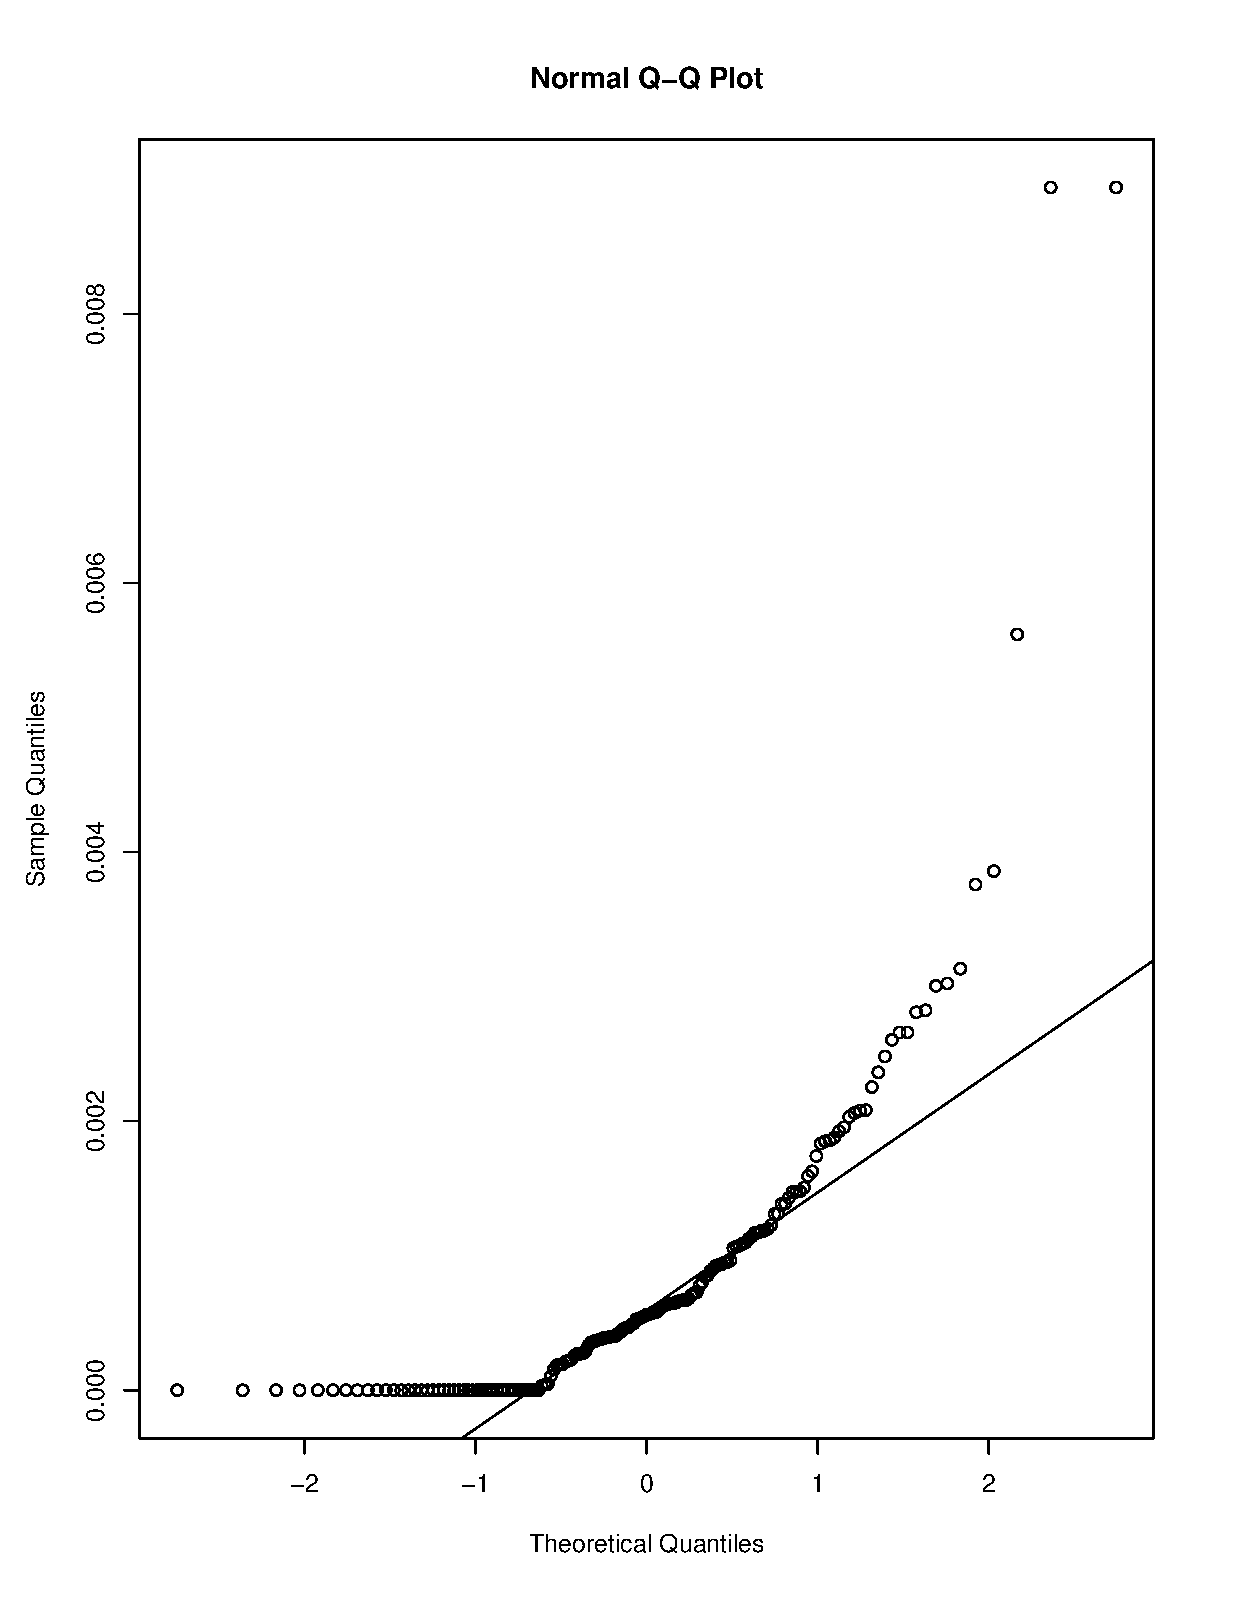
\includegraphics[width=0.8\textwidth]{qq}
  \caption{Q-Q plot for CTR\% \label{fig:qq}}
\end{figure}

We also used Shapiro-Wilk normality test. Here is the test result from R:

\begin{verbatim}
        Shapiro-Wilk normality test

data:  CTR
W = 0.652, p-value < 2.2e-16
\end{verbatim}

As we can see, the data is not normally distributed ($p-value < 0.05$). \\

{\bf 7. What combination of campaign / publisher would result in the most profitable outcome? How much performance is lost on campaign level? Constraint here is to deliver the same number of impressions for each campaign.} \\

The result is shown in is shown in Table~\ref{tab:p7}. \\

\begin{table}[ht!]
  \begin{center}
    \begin{tabular}{|c|c|c|c|c|c|}
      \hline
                        & Campaign1  & Campaign2  & Campaign3  & Campaign4  & Campaign5  \\ \hline
      Pub ID            & 656597     & 102102105  & 737367     & 575752     & 494948     \\ \hline
      Profit/Impression & \$0.023137 & \$0.000584 & \$0.004376 & \$0.001874 & \$0.000008 \\ \hline
      Combination CTR\% & 5.263158\% & 0.360068\% & 1.179111\% & 0.512821\% & 0.064870\% \\ \hline
      Campaign CTR\%    & 0.151915\% & 0.060012\% & 0.334134\% & 0.121817\% & 0.062189\% \\ \hline
      Campaign Lvl Loss & 5.111243\% & 0.300056\% & 0.844977\% & 0.391004\% & 0.002681\% \\ \hline
    \end{tabular}
  \end{center}
  \caption{The most profitable combination \label{tab:p7}}
\end{table}

First, we calculated the "Profit / Impression" for each "campaign / publisher" combination. The result is listed in spreadsheet "P7". Then we find out the most profitable combination for each campaign, as shown in Table~\ref{tab:p7}. \\

For Campaign level performance loss, here is the formula:
\begin{eqnarray*}
\text{Campaign Level Loss} = \text{Combination CTR\%} - \text{Campaign CTR\%}
\end{eqnarray*}

That is, if we put all the advertises of each campaign to the publisher which generates the greatest profit to that campaign, how much performance we will gain. In other words, how much performance we have lost on campaign level. \\

Note that for this solution, the underlying assumption is that each publisher's impression number is unlimited. That is, we can get any impression number we want from each publisher. In this way, we can launch our campaign on solely one publisher. \\

{\bf 8. While OurCompany's goal is to maximize profit, advertisers' monitor performance and ROI. Having multiple goals in mind, how would you allocate campaigns across publishers? Constraint here is to deliver the same number of impressions for each campaign.} \\

There are three factors we want to consider: "Profit / Impression", "CTR\%" and "ROI". \\

For each factor, we give a separate rank for each "campaign / publisher" combination. In this way, we make the numeric value of three different factors comparable. \\

Intuitively, we want to choose a "campaign / publisher" combination with considering three different factors. If there's a "campaign / publisher" combination that ranks $1st$ in "Profit / Impression", "CTR\%" and "ROI", then it is definitely the best we want to choose. \\

Now we use the three ranks to give our final evaluation formula:
\begin{eqnarray*}
f(x) = \omega_1 \cdot Rank(\text{Profit / Impression}) + \omega_2 \cdot Rank(\text{CTR\%}) + \omega_3 \cdot Rank(\text {ROI})
\end{eqnarray*}

Note that $\omega_1$, $\omega_2$ and $\omega_3$ are arbitrary. It depends on which factor we care more. But there is one constraint:
\begin{eqnarray*}
\omega_1 + \omega_2 + \omega_3 = 1
\end{eqnarray*}

Here we use
\begin{eqnarray*}
\omega_1 &=& 1/3 \\
\omega_2 &=& 1/3 \\
\omega_3 &=& 1/3 
\end{eqnarray*}

With formula $f(x)$, we can evaluate each "campaign / publisher" combination. All the $f(x)$ is listed in spreadsheet "P8" of file "dataset.xlsx". \\

Note that about the rank in spreadsheet "P8", rank with value 1 is the lowest rank. \\

***** NOT FINISHED: NEED DISCUSSION HERE ***** \\

{\bf 9. In your opinion, what is the purpose of data segments?} \\

Data segments help improving the performance of an advertisement. \\

Data segments make adverting targeted. That is, data segments help advertisement more easily to reach the targeted population, who is more likely to convert from advertising. In the sense of CTR\%, targeted advertising tends to have a higher CTR\%. \\

That is, data segments improve the CTR\%, or in general, the performance. \\

{\bf 10. You are now launching a new campaign that needs to use RON and Automotive data segments. How would you go about distributing the campaign across the publishers?} \\

Similar to question 8, for each "publisher / segment" combination, we give the following formula to do the evaluation:
\begin{eqnarray*}
f(x) = \omega_1 \cdot Rank(\text{Profit / Impression}) + \omega_2 \cdot Rank(\text{CTR\%}) + \omega_3 \cdot Rank(\text {ROI})
\end{eqnarray*}

Still, $\omega_1$, $\omega_2$ and $\omega_3$ are arbitrary so long as
\begin{eqnarray*}
\omega_1 + \omega_2 + \omega_3 = 1
\end{eqnarray*}

In Particular, we use the following weight:
\begin{eqnarray*}
\omega_1 &=& 1/3 \\
\omega_2 &=& 1/3 \\
\omega_3 &=& 1/3
\end{eqnarray*}

All the $f(x)$ are listed in spreadsheet "P10" of file "dataset.xlsx". \\

Having the $f(x)$ for each "publisher / segment" combination, we choose publishers from the one with highest $f(x)$, the second highest $f(x)$, and so on. \\

{\bf 11. If one were to rank campaigns on each publisher for priority, how would you suggest ranking be done? What additional data you would need as your input parameters?} \\

To rank campaigns on each publisher for priority, there are three factors we want to consider: "Profit / Impression", "CTR\%" and "ROI". \\

Similar to question 8, for each factor, we give a separate rank for each "campaign / publisher" combination. Then we use the three ranks to give our final evaluation formula:
\begin{eqnarray*}
f(x) = \omega_1 \cdot Rank(\text{Profit / Impression}) + \omega_2 \cdot Rank(\text{CTR\%}) + \omega_3 \cdot Rank(\text {ROI})
\end{eqnarray*}

There is one constraint:
\begin{eqnarray*}
\omega_1 + \omega_2 + \omega_3 = 1
\end{eqnarray*}

Note that $\omega_1$, $\omega_2$ and $\omega_3$ are arbitrary so long as their sum is 1. It depends on which factor we care more. So, the extra input for this question we need is weight $\omega_1$, $\omega_2$ and $\omega_3$. \\

At last, the $f(x)$ is the priority we give to each "campaign / publisher" combination, the higher the $f(x)$ is, the higher its priority is. \\

Particularly, we use the following weights:
\begin{eqnarray*}
\omega_1 &=& 1/3 \\
\omega_2 &=& 1/3 \\
\omega_3 &=& 1/3
\end{eqnarray*}

All the priorities based on these weights are listed in spreadsheet "P11\_Priority" of file "dataset.xlsx". \\

\end{document}
